% Created 2017-08-30 Wed 15:02
\documentclass[presentation]{beamer}
\usepackage[utf8]{inputenc}
\usepackage[T1]{fontenc}
\usepackage{fixltx2e}
\usepackage{graphicx}
\usepackage{longtable}
\usepackage{float}
\usepackage{wrapfig}
\usepackage{rotating}
\usepackage[normalem]{ulem}
\usepackage{amsmath}
\usepackage{textcomp}
\usepackage{marvosym}
\usepackage{wasysym}
\usepackage{amssymb}
\usepackage{hyperref}
\tolerance=1000
\setbeamertemplate{navigation symbols}{}
\usetheme{default}
\author{Week 2 - PSYC 5316}
\date{September 4, 2017}
\title{Maximum Likelihood Estimation}
\hypersetup{
  pdfkeywords={},
  pdfsubject={},
  pdfcreator={Emacs 25.2.1 (Org mode 8.2.10)}}
\begin{document}

\maketitle

\begin{frame}[label=sec-1]{Recall}
Last time, we gave a formal definition for a \alert{probability function}.  An example was the \emph{binomial} distribution for $N$ independent Bernoulli trials (e.g., coin flips):

\[
f(x\mid \theta) = {N\choose x} \theta^x(1-\theta)^{N-x}
\]

where $x$ = \# of successes, and $\theta$ = probability of success.
\end{frame}

\begin{frame}[fragile,label=sec-2]{Probability function}
 Suppose $N=20$ and $\theta=0.7$.  

\begin{verbatim}
barplot(dbinom(0:20,size=20,prob=0.7),
        names.arg=0:20,
        ylab="p(x)",
        xlab="x")
\end{verbatim}

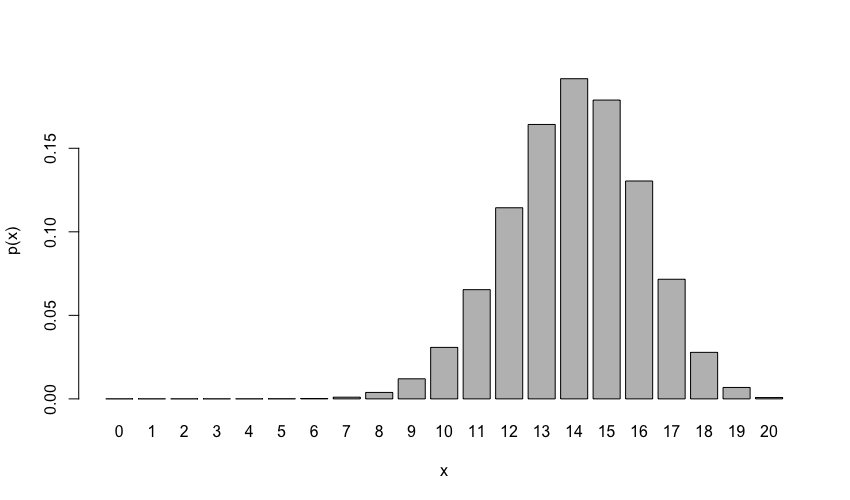
\includegraphics[width=.9\linewidth]{figures/week2/binom.png}
\end{frame}

\begin{frame}[label=sec-3]{Data and parameters}
\[
f(x\mid \theta) = {N\choose x} \theta^x(1-\theta)^{N-x}
\]

\vspace{1cm}

This function gives us the probability of \alert{data}, \emph{given} a specific \alert{parameter}
\end{frame}


\begin{frame}[label=sec-4]{Data and parameters}
What if we switched these?

\[
f(\theta \mid x) = {N\choose x} \theta^x(1-\theta)^{N-x}
\]

\vspace{1cm}

This function then gives us the likelihood of a range of \alert{parameters}, \emph{given} a specific \alert{data point}
\end{frame}

\begin{frame}[fragile,label=sec-5]{Likelihood function}
 Suppose we observed 12 successes in 20 trials:

\begin{verbatim}
theta=seq(from=0, to=1, by=0.01)
plot(theta, dbinom(x=12, size=20, prob=theta), 
     type="l",ylab="likelihood")
\end{verbatim}

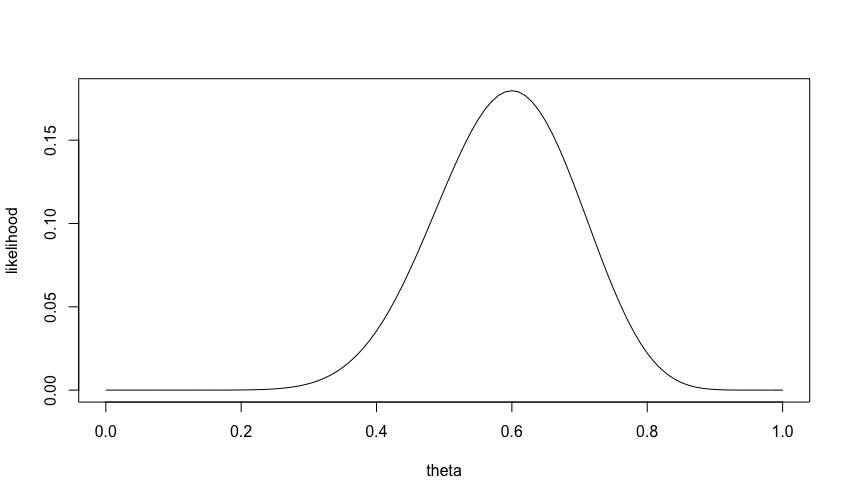
\includegraphics[width=.9\linewidth]{figures/week2/likelihood.png}
\end{frame}


\begin{frame}[label=sec-6]{Likelihood function}
Suppose we observed 12 successes in 20 trials:

\vspace{1cm}

Natural question -- what value of $\theta$ is \alert{most likely}, given the data?

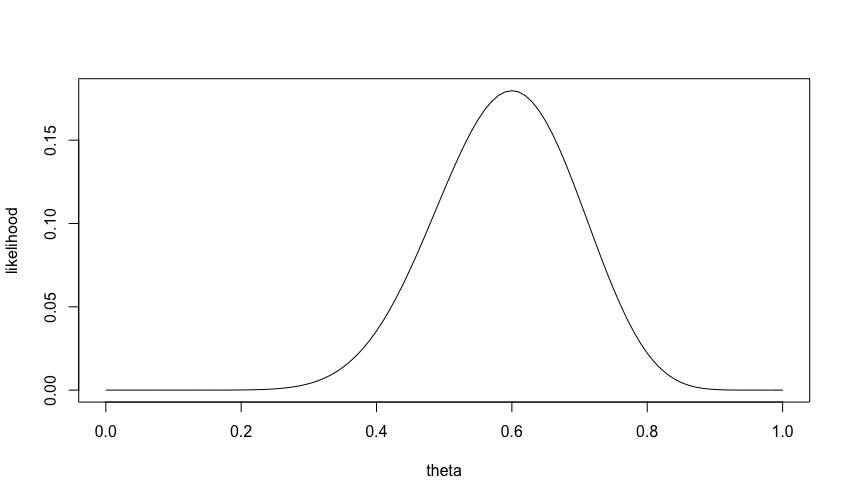
\includegraphics[width=.9\linewidth]{figures/week2/likelihood.png}
\end{frame}


\begin{frame}[label=sec-7]{Likelihood function}
Suppose we observed 12 successes in 20 trials:

\vspace{1cm}

Natural question -- what value of $\theta$ is \alert{most likely}, given the data?

Answer: $\theta=0.6$

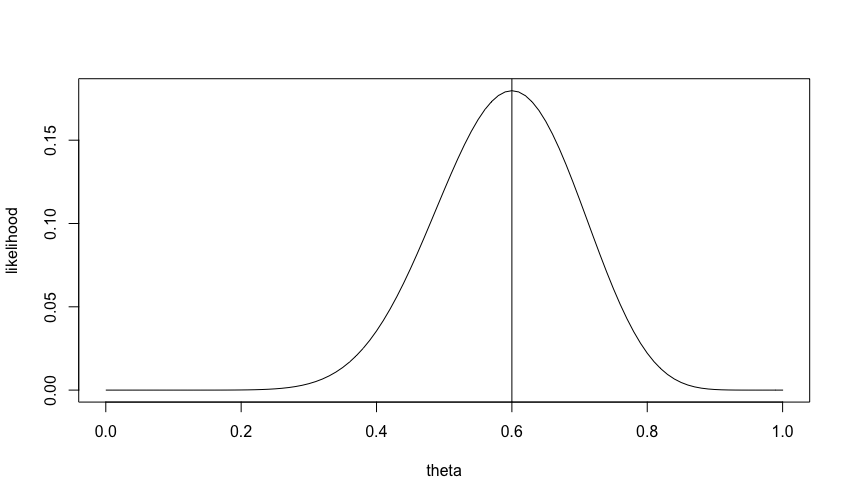
\includegraphics[width=.9\linewidth]{figures/week2/maxLikelihood.png}
\end{frame}

\begin{frame}[label=sec-8]{Maximum likelihood estimation}
A key problem in statistical inference is how to infer from \alert{sample data} to \alert{population parameters}.

\vspace{1cm}

Maximum likelihood estimation is one solution to this problem
\end{frame}

\begin{frame}[label=sec-9]{Maximum likelihood estimation}
Basic workflow:
\begin{enumerate}
\item collect data
\item decide on a "model" for the data (e.g., binomial, normal, etc.)
\item define a likelihood function based on the underlying model
\item find the parameter value(s) that \alert{maximize} the likelihood function
\end{enumerate}
\end{frame}
% Emacs 25.2.1 (Org mode 8.2.10)
\end{document}